\subsection*{\Large Общая характеристика работы}
\fontsize{14pt}{15pt}\selectfont

\textbf{Актуальность темы исследования.} Исследования картин мира (КМ) субъектов деятельности принадлежат одному из центральных направлений в когнитивной психологии. Высшие психические функции, в том числе связанные с приобретением и использованием знаний, являются, в широком смысле, продуктом работы КМ субъекта. Исследованию большого числа процессов, протекающих в КМ, в~том числе высших когнитивных, таких как категоризация и обобщение, целеполагание, планирование, принятие решения, творческие синтез и анализ, было посвящено значительное число работ на протяжении всей истории психологической науки. Следует отметить работы по восприятию Дж.\,А.~Фодора (J.\,A.~Fodor), Б.~Юлеза (B.~Julesz), Дж.\,Е.~Каттинга (J.\,E.~Cutting), С.~Гроссберга (S.~Grossberg), А.\,Р.~Лурия, Б.\,М.~Величковского, В.\,П.~Зинченко и памяти С.~Стернберга (S.~Sternberg), Л.~Джакоби (L.~Jacoby), Р.~Аткинсона (R.~Atkinson), Р.~Шиффрина (R.~Shiffrin), Е.~Тулвинга (E.~Tulving).

В последнее время исследованию когнитивных функций человека уделяется большое внимание не только в самой психологии, но и в нейрофизиологии и в~искусственном интеллекте. Нейрофизиологи основной своей задачей ставят поиск нейронного субстрата психических функций. При этом в качестве основного инструмента здесь выступает картирование участков коры головного мозга и отслеживание динамики активности различных участков при выполнении той или иной когнитивной задачи. Большое количество накопленного фактического материала используется для подтверждения целого ряда разрозненных моделей отдельных психических функций. Примерами могут служить работы по моделям внимания Я.\,Б.~Казановича, С.~Фринтропа (S.~Frintrop), С.~Коха (C.~Koch), Л.~Итти (L.~Itti), Дж.\,К.~Сосоза (J.\,K.~Tsotsos), А.~Торралба (A.~Torralba), Л.~Жэнга (L.~Zhang), Р.\,А.~Ренсинка (R.\,A.~Rensink). Единого аппарата для построения таких моделей на данный момент не существует, хотя имеется ряд работ Б.\,Дж.~Баарса (B.\,J.~Baars), Р.~Сана (R.~Sun), Дж.~Хокинса (J.~Hawkins), которые можно считать первыми попытками их создания.

Искусственный интеллект в начале своего становления как науки использовал для построения интеллектуальных алгоритмов данные психологов. Однако спустя некоторое время психологические соображения уже перестали рассматриваться как определяющие при разработке того или иного алгоритма. Центральное место стали занимать вопросы вычислительной эффективности и специализации в той или иной предметной области. В~связи с~тем, что в~большинстве интеллектуальных систем в~настоящее время требуется всё большая степень универсальности и автономности, начинается процесс возвращения к психологическим основам строения психики человека. Возникает задача построения моделей процессов, например, распознавания и планирования, на некоторой <<биологически инспирированной основе>>. К этому направлению относятся работы Дж.\,Р.~Андерсона (J.\,R.~Anderson), П.~Леирда (J.\,E.~Laird), П.~Ленгли (P.~Langley). Подтверждением повышенного интереса к этой теме служат организуемые в последнее время конференции и издаваемые журналы, посвящённые исключительно <<биологически правдоподобным>> архитектурам (например, ежегодные конференции BICA (Annual International Conference on Biologically Inspired Cognitive Architectures)\footnote{BICA Society. BICA 2014."--- 2014."--- URL: http://bicasociety.org/meetings/2014/ (дата	обращения: 01.02.2015).} и журнал BICA \footnote{Elsevier. Biologically Inspired Cognitive Architectures "--- Journal."--- 2015."---
URL: http://www.journals.elsevier.com/biologically-inspired-cognitive-architectures/ (дата	обращения: 01.02.2015).}).

Потребность в единой модели КМ субъекта деятельности для нейрофизиологов и исследователей в области искусственного интеллекта определяет актуальность данной работы. Такая модель требуется как для построения моделей когнитивных функций человека на нейронном уровне, подтверждаемых нейрофизиологическими данными о строении высшей нервной системы человека и данными об активности соответствующего определённой функции участка коры головного мозга, так и для построения абстрагированных от того или иного субстрата интеллектуальных алгоритмов, которые могли бы быть использованы в автономных системах свободной конфигурации.

Один из основных вопросов, возникающих при разработке модели КМ, заключается в описании базовых элементов картины мира и построении алгоритма их формирования в процессе деятельности субъекта "--- носителя КМ. В качестве психологической основы для построения модели элемента КМ были использованы, с одной стороны, культурно"--~исторический подход Л.\,Н.~Выготского и теория деятельности А.\,Н.~Леонтьева, с другой стороны "--- идеи прикладной семиотики, предложенные в работах Д.\,А.~Поспелова, А.~Мейстеля, Г.\,С.~Осипова. В качестве нейрофизиологических предпосылок были использованы концепции и нейронные схемы Д.~Георга (D.~George).

\textbf{Предмет исследования} "--- знаковые модели картины мира и некоторых когнитивных функций субъекта деятельности.

\textbf{Целью исследования} является разработка моделей и алгоритмов формирования элементов знаковой картины мира, обладающих структурой, необходимой для построения моделей высших когнитивных функций, в том числе восприятия, внимания, планирования и целеполагания.

Для~достижения цели работы были поставлены следующие \textbf{задачи}:
\begin{enumerate}
	\item исследовать модель элементов картины мира субъекта, построенную на основе психологической теории деятельности;
	\item построить модель структурных компонент элементов картины мира, опирающуюся на нейрофизиологические данные, и исследовать её;
	\item исследовать структуру отношений и процессы самоорганизации на множестве элементов картины мира на синтаксическом уровне;
	\item исследовать процесс формирования и связывания основных компонент нового элемента картины мира и построить соответствующий алгоритм;
	\item исследовать сходимость процесса формирования и связывания основных компонент нового элемента картины мира.
\end{enumerate}

\textbf{Научная новизна и результаты, выносимые на~защиту.}
\begin{enumerate}
	\renewcommand\labelenumi{\theenumi.}
	\item Впервые построена модель структурных компонент элементов картины мира субъекта деятельности.
	\item Построены операторы распознавания в статическом, динамическом и иерархическом случаях в терминах алгебраической теории для образной компоненты элемента картины мира.
	\item Доказаны теоремы корректности линейных замыканий множеств построенных в работе операторов распознавания.
	\item Построен алгоритм формирования и связывания основных компонент нового элемента картины мира.
	\item Доказана сходимость процесса формирования и связывания основных компонент нового элемента картины мира.
\end{enumerate}

\textbf{Практическая значимость.} Построение модели элементов картины мира субъекта деятельности, с~одной стороны, позволит создать универсальные интеллектуальные алгоритмы планирования поведения, целеполагания, локализации, распознавания и категоризации, применение которых в интеллектуальных системах повысит степень их автономности, а с~другой стороны, позволит объяснить некоторые патологические явления в мозге человека и дать рекомендации к их устранению.

\textbf{Методы исследования.} Теоретические результаты работы получены и обоснованы с использованием методов теории множеств, алгебраической теории распознавания образов, теории интеллектуальных динамических систем, теории деятельности.

\textbf{Достоверность результатов} подтверждена строгими математическими доказательствами утверждений и результатами вычислительных экспериментов.

\textbf{Апробация результатов исследования.} Основные результаты работы докладывались~на: Международных конференциях по когнитивной науке (Томск, 2010~г.; Калининград, 2012~г., 2014~г.), II~Всероссийской научной конференции молодых учёных с международным участием <<Теория и практика системного анализа>> (Рыбинск, 2012~г.), IV~Международной конференции <<Системный анализ и информационные технологии>> (Абзаково, 2011~г.), V~съезде Общероссийской общественной организации <<Российское психологическое общество>> (Москва, 2012~г.), X~Международной конференции <<Интеллектуализация обработки информации>> (Крит, 2014~г.), I~конференции Международной ассоциации когнитивной семиотики (Лунд, 2014~г.), Общемосковском научном семинаре <<Проблемы искусственного интеллекта>>, на семинарах ИСА~РАН и ВЦ~РАН.

\textbf{Публикации.} Основные результаты по теме диссертации изложены в 14 печатных работах, 4 из которых изданы в рецензируемых журналах из списка ВАК~РФ, 7 "--- в материалах всероссийских и международных конференций.

\textbf{Объем и структура работы.} Диссертация состоит из~введения, трёх глав, заключения и~двух приложений. Полный объём диссертации составляет 118 страниц с 23 рисунками. Список литературы содержит 81 наименование.

\newpage
\subsection*{\Large Краткое содержание работы}
Во \textbf{введении} обоснована актуальность темы, определён предмет исследования, сформулированы цель и задачи исследования, научная новизна, практическая значимость полученных результатов, а также приведены данные о структуре и объёме диссертации.

В \textbf{первой главе} приведён обзор существующих теорий и моделей, которые послужили предпосылками для создания общей модели картины мира субъекта деятельности. Даётся описание психологических предпосылок: культурно"--~исторического подхода Л.\,С.~Выготского \footnote{Выготский~Л.\,С. Психология развития человека."--- М. : Издательство Смысл, 2005."---	С. 1136.}, теории деятельности А.\,Н.~Леонтьева \footnote{Леонтьев~А.\,Н. Деятельность. Сознание. Личность."--- М. : Политиздат, 1975.} и модели психики Е.\,Ю.~Артемьевой \footnote{Артемьева~Е.\,Ю. Психология субъективной семантики."--- М. : Издательство МГУ, 1980.}. Приводятся и направления исследований, проводящихся по данной теме за рубежом.

Вторая часть главы посвящена краткому обзору нейрофизиологических исследований. Особое внимание уделяется глобальным моделям, в которых делается попытка описать не только отдельную когнитивную функцию, а целую их систему. Подробно описываются основные положения теории повторного входа Д.\,М.~Эдельмана \footnote{Edelman~G.\,M. Neural Darwinism: The Theory Of Neuronal Group Selection."--- New York : Basic Books, 1987."--- P. 400.}, теории информационного синтеза А.\,М.~Иваницкого \footnote{Иваницкий~А.\,М. Мозговая основа субъективных переживаний: гипотеза информационного синтеза // Журнал высшей нервной деятельности."--- 1996."---	Т. 46, \No 2."--- С. 241--282.}, теории глобального рабочего пространства Б.\,Дж.~Баарса с его нейронной реализацией по С.~Дехане \footnote{Dehaene~S., Sergent~C., Changeux~J.\,P. A neuronal network model linking subjective reports and objective physiological data during conscious perception // Proceedings of National	Academy of Sciences USA."--- 2003."--- Vol. 100, no. 14."--- P. 8520--8525.}, а также модель иерархической временной памяти в представлении Дж.~Хокинса и Д.~Георга \footnote{George~D., Hawkins~J. Towards a Mathematical Theory of Cortical Micro-circuits // PLoS Computational Biology."--- 2009."--- Vol. 5, no. 10."--- P. 1--26.}.

В заключении первой главы приводится краткий обзор идей прикладной семиотики, в которой впервые была определена важная роль семиотических (знаковых) описаний для решения важных проблем искусственного интеллекта. В истоках этого подхода стояли Д.\,А.~Поспелов, Г.\,С.~Осипов, А.\,М.~Мейстель.

Во \textbf{второй главе} вводится формальное определение знака "--- базового элемента картины мира "--- и описывается синтаксический уровень модели картины мира субъекта деятельности.

Даётся описание компонент знака по Леонтьеву и приводится алгоритм формирования нового знака. Следуя теории деятельности представление каждого объекта или процесса в картине мира включает три компоненты: \textit{образ} явления, его \textit{значение} и \textit{личностные смыслы} субъекта, связанные с этим явлением. До момента связывания в знак три компоненты называются \textit{перцептом}, \textit{биологическим смыслом} и \textit{функциональным значением} соответственно. Связывание упомянутых трёх компонент в единую структуру позволяет перейти к рассмотрению явления как целостного и существующего независимо от текущего состояния действующего субъекта. Такое связывание становится возможным благодаря именованию возникающей структуры, что приводит к конструкции, называемой \textit{знаком}.

Процесс формирования (актуализации) знака выглядит следующим образом:
\begin{enumerate}
	\setcounter{enumi}{-1}
	\renewcommand\labelenumi{\theenumi.}
	\item\label{step0} \textit{Локализация} явления в пространстве, времени и измерении значений \footnote{Леонтьев А. Н. Избранные психологические произведения. Том II."--- М. : Педагогика,
		1983."--- С. 251--261.}.
	\item\label{step1} \textit{Формирование} перцепта, основанное на работе процедуры воспроизведения свойств явления моторикой воспринимающего органа (для живых существ) или на обработке методами распознавания образов информации, снимаемой с датчиков (для искусственных систем).
	\item\label{step2} \textit{Порождение} на основе прошлого опыта или на основе прецедентов, представленных в виде множества пар <<перцепт "--- функциональное значение>>, и сформированного на шаге \ref{step1} перцепта "--- нового функционального значения явления.
	\item\label{step3} \textit{Оценка} специальным механизмом степени близости функционального значения, полученного на стадии \ref{step2} к функциональному значению, полученному на стадии \ref{step0}; в случае недостаточной близости "--- переход к шагу \ref{step1} и продолжение формирования перцепта (в психологии сенсорно"--~перцептивных процессов этот механизм получил название <<сенсорная уверенность>>).
	\item\label{step4} Стадии \ref{step1}--\ref{step3} выполняются до получения степени близости, достаточной с точки зрения специального механизма, упомянутого на шаге \ref{step3}.
	\item\label{step5} \textit{Получение} субъектом из культурно"--~исторической среды, аккумулированной в системе естественного языка, пары <<имя знака "--- значение>> и оценка специальным механизмом степени близости функционального значения, построенного на стадии \ref{step4} к значению, полученному из культурной среды; в случае недостаточной близости "--- переход к шагу \ref{step1} и продолжение формирования перцепта.
	\item\label{step6} \textit{Связывание} имени из пары <<имя знака "--- значение>> с перцептом, построенным после завершения выполнения шагов \ref{step1}--\ref{step5}. С этого момента перцепт превращается в образ.
	\item \textit{Формирование} личностных смыслов знака на основе прецедентов действий с явлением.
	\item \textit{Связывание} имени из пары <<имя знака "--- значение>> со сформированным личностным смыслом. С этого момента функциональное значение превращается в значение, а биологический смысл "--- в личностный смысл.
	\item \textit{Продолжение} отображения <<биологический смысл "--- перцепт>> включением в область определения отображения личностного смысла, полученного в предыдущем пункте, а в область значений "--- образа из шага \ref{step6}.
\end{enumerate}

Вводятся обозначения для компонент знака:  $a\subseteq A$ "--- подмножество множества личностных смыслов (возможно пустое), $m\subseteq M$ "--- подмножество множества значений (функциональных либо культурно"--~исторических), $p\subseteq P$ "--- подмножество множества признаков (перцепт либо образ) (Рисунок \ref{fg:sign}).
\begin{figure}[h]
	\centering
	\begin{subfigure}[b]{0.45\textwidth}
		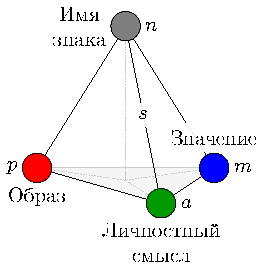
\includegraphics[width=0.9\linewidth]{signs/sign_colored}
		\caption{}
		\label{fg:sign}
	\end{subfigure}
	~
	\begin{subfigure}[b]{0.45\textwidth}
		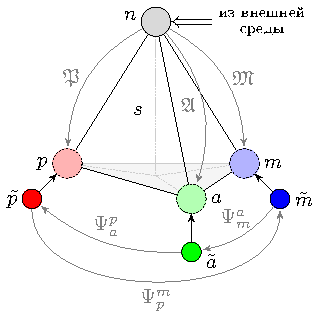
\includegraphics[width=0.9\linewidth]{signs/sign_naming_colored}
		\caption{}
		\label{fg:sign_naming}
	\end{subfigure}
	\caption{Знак и его структура.}
\end{figure}

Далее вводятся специальные \textit{отображения связывания}. Первое из таких отображений $\Psi_p^m:2^P\rightarrow 2^M$ "--- процедура связывания образа (или перцепта) $p$ с (функциональным) значением $m$ так, что $\Psi_p^m(p^{(i)})=m^{(i)}$, где $i$ "--- номер итерации, $p^{(i)}\in 2^P$, $m^{(i)}\in 2^M$, $2^P$ и $2^M$ "--- булеаны $P$ и $M$ соответственно.

Второе отображение $\Psi_m^a:2^M\rightarrow 2^A$ связывает значения (или функциональные значения) с личностными (или биологическими) смыслами таким образом, что $\Psi_m^a(m^{(i)})=a^{(i)}$, где $m^{(i)}\in 2^M$, $a^{(i)}\in 2^A$, $2^A$ "--- булеан $A$. Отображение $\Psi_a^p:2^A\rightarrow 2^P$ связывает личностные (или биологические) смыслы с образом (перцептом) так, что $\Psi_a^p(a^{(i)})=p^{(i+1)}$, где $a^{(i)}\in 2^A$, $p^{(i+1)}\in 2^P$.

С помощью введённых отображений описывается процесс связывания функционального значения и образа восприятия на основе элементарных топологических соображений.

Наконец, во второй главе вводятся функции, связывающие имя и компоненты знака: функция $\mathfrak M(n)$, выдающую по имени $n$ значение $m$, и аналогичные функции для образа $\mathfrak P(n)$ и личностного смысла $\mathfrak A(n)$ (Рисунок \ref{fg:sign_naming}). Доказываются следующие утверждения:

\begin{Pred}
	\label{pred:fixed_point}
	Если $s$ "--- знак, $p$, $m$, $a$ "--- его образ, значение и личностный смысл, соответственно, то тройка $\langle p,m,a\rangle$ есть неподвижная точка оператора $\Psi_a^p\Psi_m^a\Psi_p^m$.
\end{Pred}

\begin{Pred}
	Если $s$ "--- знак, то  $\Psi_m^a\Psi_p^m\Psi_a^p$, $\Psi_a^p\Psi_m^a\Psi_p^m$ и $\Psi_p^m\Psi_a^p\Psi_m^a$ "--- тождественные операторы.
\end{Pred}

\begin{Pred}
	Если $s$ "--- знак, то $\Psi_p^m(\mathfrak P(n))=\mathfrak M(n)$, $\Psi_m^a\Psi_p^m(\mathfrak P(n))=\mathfrak A(n)$.
\end{Pred}	

В заключении второй главы описываются отношения на множестве компонент знака и процессы самоорганизации на множестве знаков. На синтаксическом уровне образ представляется в виде набора признаков, что позволяет на множестве образов ввести следующие бинарные отношения: эквивалентности $R_1$, включения $R_2$, сходства $R_3$ и противопоставления $R_4$, а также описать операцию обобщения $\Theta$.

Личностные смыслы определяются через множество действий. На множестве личностных смыслов вводятся отношения поглощения $\sqsubseteq$, противопоставления $\perp$ и агглютинации $\sqcup$. Наконец, элемент значения на синтаксическом уровне представ\'{и}м в виде предикатного слова и некоторой определённой семантической валентности. На множестве значений вводятся отношения эквивалентности $R'_1$, сходства $R'_3$, ситуационное $R_6$ и сценарное $R_7$ отношения.

\textbf{Третья глава} посвящена описанию семантического уровня модели картины мира субъекта деятельности. В начале главы приводятся основные принципы работы образной компоненты знака и определяется бесконечный автомат Мили с переменной структурой и конечной памятью 

\[
R_i^j=<X_i^j\times \hat{X}_i^{j+1}, 2^{\mathcal Z_i^j}, X_i^{*j}\times \hat{X}_i^j,\varphi_i^j,\vec\eta_i^j,>,
\]
где
\begin{itemize}
	\item $X_i^j$ "--- множество входных сигналов (пространство векторов длины $q_i^j$ действительных чисел от $0$ до $1$), 
	\item $X_i^{*j}$ "--- множество выходных сигналов (пространство векторов длины $l_i^j$ действительных чисел от $0$ до $1$), 
	\item $\hat{X}_i^{j+1}$ "--- множество управляющих сигналов с верхнего уровня иерархии (пространство векторов длины $l_i^j$ действительных чисел от $0$ до $1$),
	\item $\hat{X}_i^j$ "--- множество управляющих сигналов на нижний уровень иерархии (пространство векторов длины $q_i^j$ действительных чисел от $0$ до $1$),
	\item $2^{\mathcal Z_i^j}$ "--- множество состояний (булеан матриц предсказания),
	\item $\varphi_i^j:X_i^j\times \hat{X}_i^{j+1}\to 2^{\mathcal Z_i^j}$ "--- функция переходов,
	\item $\vec\eta_i^j:2^{\mathcal Z_i^j} \to X_i^{*j}\times \hat{X}_i^j$ "--- вектор"--~функция выходов.
\end{itemize}

Такой автомат, функционирующий по определённому нейрофизиологически правдоподобному алгоритму $\mathfrak A_{th}$ (см. стр. \pageref{alg:th_init} и \pageref{alg:th_cycle}), называется \textit{распознающим} или\textit{ $R$-автоматом}. Здесь и далее $\omega_i^j:T{\to}X_i^j$ "--- входное воздействие, а $\gamma_i^j:T{\to}X_i^{*j}$ "--- выходная величина. Алгоритм работы распознающего автомата моделирует работу образной компоненты знака. Множество $R$-автоматов образуют иерархию (верхний индекс в обозначении автомата "--- уровень иерархии, нижний "--- сквозной индекс по множеству).

\begin{algorithm}[h]
	\caption{Алгоритм $\mathfrak{A}_{th}$ (часть I, задание начального состояния)}\label{alg:th_init}
	\begin{algorithmic}[1]
				\Require $\tau_s, \hat{x}_i^{j+1}(\tau_s), \omega_i^j$.
		\Ensure $\varphi_{i\Delta t}^j, \vec\eta_{i\Delta t}^j$.

		\State $\hat{F}^*=\varnothing,Z^*=\varnothing,t=0$; \Comment{активные функции распознавнаия и матрицы предсказания}
		\State $c_1\in(0,1), c_2\in(0,1)$; \Comment{пороговые константы}

		\Statex \Comment{определение начального состояния}
				
		\ForAll{компонент $\hat{x}_{ik}^{j+1}$ вектора $\hat{x}_i^{j+1}(\tau_s)=(\hat{x}_{i1}^{j+1},\hat{x}_{i2}^{j+1},\dots,\hat{x}_{il}^{j+1})$} \label{alst:init_start}
			\If{$\hat{x}_{ik}^{j+1}{\ge}c_1$} \label{alst:select_f}
				\State $\hat{F}^*:=\hat{F}^*\cup\{\hat{f}_k\}$;
			\EndIf
		\EndFor
		
		\State $\bar x_i^j:=\omega_i^j(\tau_s)$;
		
		\ForAll{функций распознавания $\hat{f}_k\in\hat{F}^*$}
			\ForAll{$Z_r^k\in Z_k$, соответствующих функции распознавания $\hat{f}_k$,}
				\If{$\frac{\|\bar{z}_1^r-\bar{x}_i^j\|}{\|\bar{z}_1^r\|+\|\bar{x}_i^j\|}<c_2$} \label{alst:select_z}
					\State $Z^*:=Z^*\cup\{Z_r^k\}$;
				\EndIf
			\EndFor
		\EndFor
		
		\State $\varphi_i^j(\bar x_i^j,\hat{x}_i^{j+1}(\tau_s)) := Z^*$; \Comment{значение функции переходов в начальный момент времени}\label{alst:init_state}
		\State $\bar N:=(|\{Z_r^1|Z_r^1\in Z^*\}|,\dots,|\{Z_r^{l_i^j}|Z_r^{l_i^j}\in Z^*\}|)$; \label{alst:init_calc_out2}
		\State $\eta(Z^*)=\bar{x}_i^{*j}:=W(\bar N)$; \Comment{значение функции выходов в начальный момент времени} \label{alst:init_calc_out3}
		\State $\hat x_i^j=W(\sum_{\hat f_k\in\hat F^*}\hat x_{ik}^{j+1}\sum_{Z_r^k\in Z^*}\bar z_2^r)$;\label{alst:init_control}
		\label{alst:init_end}
		\algstore{algst:store1}
	\end{algorithmic}
\end{algorithm}

\begin{algorithm}[h]
	\caption{Алгоритм $\mathfrak{A}_{th}$ (часть II, основной цикл)}\label{alg:th_cycle}
	\begin{algorithmic}[1]
		\algrestore{algst:store1}
			\Statex \Comment{основной цикл}
	
	\State $t=1$;
	\While{$t\leqslant{h_i^j}-1$} \label{alst:cycle_start}
		\State $\bar{x}_i^j:=\omega(\tau_s+t)$;
	
		\ForAll{матриц предсказания $Z_r^k$ из множества $Z^*$}
			\If{$\frac{\|\bar{z}_{t+1}^r-\bar{x}_i^j\|}{\|\bar{z}_{t+1}^r\|+\|\bar{x}_i^j\|}\geqslant{c_2}$} \label{alst:update_z}
				\State $Z^*:=Z^*\setminus\{Z_r^k\}$;
			\EndIf
		\EndFor
	
		\State $\varphi_i^j(\bar x_i^j,\hat{x}_i^{j+1}(\tau_s)) := Z^*$; \Comment{значение функции переходов в момент времени $t$}
		\State $\bar N=(|\{Z_r^1|Z_r^1\in Z^*\}|,\dots,|\{Z_r^{l_i^j}|Z_r^{l_i^j}\in Z^*\}|)$; \label{alst:calc_out1}
		\State $\eta(Z^*)=\bar{x}_i^{*j}:=W(\bar N)$;\Comment{значение функции выходов в момент времени $t$} \label{alst:calc_out3}
	
		\State $t=t+1$;
		\If{$t\leqslant{h}_i^j-2$}
			\State $\hat{x}_i^j:=W(\sum_{\hat f_k\in\hat F^*}\hat x_{ik}^{j+1}\sum_{Z_r^k\in Z^*}\bar z_t^r)$; \label{alst:calc_state1}
		\EndIf
	\EndWhile \label{alst:cycle_end}
	\end{algorithmic}
\end{algorithm}

В третьей главе для обоснования корректности построенного алгоритма работы образной компоненты знака, ставится рад задач распознавания (классификации) и строится семейство операторов распознавания. Корректность алгоритма демонстрируется за счёт корректности линейных замыканий множеств построенных операторов распознавания.

В начале фиксируется момент времени $t$, равный началу некоторого $s$-го вычислительного цикла $\tau_s$ распознающего автомата, т.~е. рассматривается первый этап алгоритма $\mathfrak A_{th}$ "--- задание начального состояния $R$-автомата. В этом случае, $R$-автомат $R$ можно рассматривать как статический оператор распознавания $R(\hat x^{j+1}(\tau_s),\mathcal Z,\bar x(\tau_s))=R(\hat x^{j+1},\mathcal Z,\bar x)=\bar x^*$.

Пусть
\begin{itemize}
	\item $\mathcal Q$ "--- совокупность задач классификации,
	\item $\mathcal A$ "--- множество алгоритмов, переводящих пары $(\hat{x},\bar{x})$ в векторы $\bar{\beta}$, составленные из элементов $0,1,\Delta:A(\hat{x},\bar{x})=\bar{\beta}$.
\end{itemize}

Задача $Q(\hat{x},\bar{x},\bar\alpha)\in\mathcal Q$ состоит в построении алгоритма, вычисляющего по поступившему вектору ожиданий $\hat{x}$ и входному вектору $\bar{x}$ информационный вектор $\bar\alpha=(\alpha_1,\dots,\alpha_l)$, значения которого $\alpha_i\in\{0,1\}$ являются оценками  признаков $f_1^*,…,f_l^*$.

\begin{Def}
	Алгоритм $A$ называется корректным для задачи $Q$, если выполнено равенство
	$$
	A(\hat{x},\bar{x})=\bar{\alpha}.
	$$
	Алгоритм $A$, не являющийся корректным для $Q$, называется некорректным.
\end{Def}

\begin{Pred}[аналог теоремы Ю.\,И.~Журавлёва о введении пространства оценок]\label{st:decompositon}
	Каждый алгоритм $A\in\mathcal A$ представ\'{и}м как последовательность выполнения алгоритмов $R$ и $C$, где $R(\hat{x},\bar{x})=\bar{x}^*$, $\bar{x}^*$ "--- вектор действительных чисел, $C(\bar{x}^*)=\bar{\beta}$, $\beta_i\in\{0,1,\Delta\}$.
\end{Pred}
$R$ называется оператором распознавания, а $C$ "--- решающим правилом.

\begin{Def}
	Решающее правило $C^*$ называется корректным на множестве входных векторов $X$, если для всякого вектора $\bar x$ из $X$ существует хотя бы один числовой вектор $\bar x^*$ такой, что $C^*(\bar{x}^*)=\bar{\alpha}$, где $\bar{\alpha}$ "--- произвольный информационный вектор входного вектора $\bar{x}$.
\end{Def}
На множестве операторов $\mathcal R$ вводятся операции умножения на скаляр, сложения и умножения. Пусть $r'$ "--- скаляр, $R',R''\in\mathcal R$, тогда операторы $r'{\cdot}R'$, $R'+R''$ и $R{\cdot}R''$ определяются следующим образом:
\begin{equation}
\label{eq:oper_scalar}
r'{\cdot}R'=(r'{\cdot}{x_1^*}',\dots,r'{\cdot}{x_l^*}'),
\end{equation}
\begin{equation}
\label{eq:oper_sum}
R'+R''=({x_1^*}'+{x_1^*}'',\dots,{x_1^*}'+{x_l^*}''),
\end{equation}

Доказывается следующее утверждение:
\begin{Pred}
	Замыкание $L(\mathcal R)$ множества $\mathcal R$ относительно операций \eqref{eq:oper_scalar} и \eqref{eq:oper_sum} является векторным пространством.
\end{Pred}
\begin{Def}
	Множество $L(\mathcal A)$ алгоритмов $A=R{\cdot}C^*$ таких, что $R{\in}L(\mathcal R)$, называются линейным замыканием множества $\mathcal A$.
\end{Def}

Далее фиксируется пара $(\hat{x},\bar{x})$ управляющего вектора и входного вектора и рассматриваются задачи $Q(\hat{x},\bar{x})$, обладающие следующим свойством относительно множества операторов распознавания $\mathcal{R}$.

\begin{Def}
	Если множество векторов $\{R(\hat{x},\bar{x})|R\in\mathcal R\}$ содержит базис в пространстве числовых векторов длины $l$, то задача $Q(\hat{x},\bar{x},\bar{\alpha})$ называется полной относительно $\mathcal{R}$.
\end{Def}

Имеет место следующее утверждение.
\begin{Pred}\label{st:correctness}
	Если множество задач $\mathcal Q$ состоит лишь из задач, полных относительно $\mathcal R$, то линейное замыкание $L(\{R{\cdot}C^*|R\in\mathcal R\})$ ($C^*$ "--- произвольное фиксированное корректное решающее правило) является корректным относительно $\mathcal Q$.
\end{Pred}

Далее рассматриваются только такие задачи $Q(\hat{x},\bar{x},\bar{\alpha})$, для которых удовлетворяется следующее условие: $\bar x$ не является нулевым вектором. В работе доказано следующее утверждение:
\begin{Theorem}
	\label{th:correctness}
	Линейное замыкание $L(\mathcal A)$ семейства алгоритмов $\mathcal A=\{R\cdot C^*|R\in\mathcal R\}$ с произвольным корректным решающим правилом $C^*$ и операторами распознавания $\mathcal R$, определёнными алгоритмом $\mathfrak{A}_{th}$, является корректным на $\mathcal Q$.
\end{Theorem}

Фиксация момента времени не в начале вычислительного цикла, а на~любом другом значении $\tau_s<t<\tau_s+h_i^j$, приводит к~операторам вида $R_i^j(\hat x_i^j(\tau_s), \mathcal Z_i^j, \omega_{i\Delta t}^j)$, $\Delta t=[\tau_s, t]$,  кратко $R^t$.		

Для этих операторов постановка задачи распознавания выглядит таким же образом, как и для операторов $R$, формулировки определений полноты и корректности идентичны.
Теорема о корректности линейного замыкания $L(\{R^t\cdot{C^*}|R^t\in\mathcal R^t\})$ доказывается аналогично.		

Затем рассматривается динамический случай и фиксируется не конкретный момент времени $t$, а полуинтервал ${\Delta}t=[\tau_s,\tau_s+h)$. 	В этом случае $R$-автомат $R$ можно рассматривать как \textit{динамический оператор распознавания} $\hat R(\hat x^{j+1}(\tau_s), \mathcal Z, \omega_{\Delta t})=\gamma_{\Delta t}$ принимающий  функцию входного воздействия $\omega$ и  выдающий функцию выходной величины $\gamma$. 

В этом случае задача $\hat{Q}(\hat{x}, \omega_{{\Delta}t}, \bar{\alpha})$ состоит в построении алгоритма $\hat A$, вычисляющего по поступившему начальному (управляющему) вектору ожиданий $\hat{x}$ и матрице входных воздействий $\omega_{{\Delta}t}$  информационный вектор $\bar{\alpha}$. Искомый оператор распознавания $\hat{R}$ должен выдавать весовую матрицу распознаваемых признаков $\gamma_{\Delta{t}}$, столбцы которой должны сходиться (с учётом корректного решающего правила) за $\tau_s+h$ шагов к информационному вектору $\bar\alpha$.

Т.~к. из всех столбцов выходной матрицы $\gamma_{\Delta t}$ равенство информационному вектору требуется только для последнего столбца, а на остальные накладывается некоторое ограничение, то эквивалентным по действию оператору $\hat R$ будет являться статический оператор $R^{h-1}$ со следующим ограничением на выходные векторы в моменты времени $0\leqslant t<h$:

\[
\|\bar x^*(\tau_s)-\alpha\|\geqslant \|\bar x^*(\tau_s+1)-\alpha\|\geqslant \dots\geqslant\|\bar x^*(\tau_s+h-1)-\alpha\|.
\]

Такие операторы обозначаются как $\hat R'$, а их множество соответственно $\hat{\mathcal R}'$. 

\begin{Pred}\label{st:decompositon_dyn}
	Каждый алгоритм $\hat{ A}\in\hat{\mathcal{A}}$ представ\'{и}м как последовательность выполнения алгоритмов $\hat R'$ и $\hat{C}$, где $\hat R'(\hat x, \mathcal{Z}, \omega_{\Delta{t}})=\bar x^*(\tau_s+h-1)$, $\bar x^*(\tau_s+h-1)$ "--- вектор действительных чисел, $\hat C(\bar x^*(\tau_s+h-1))=\bar\beta$, $\bar\beta$ "--- вектор значений $\beta_i\in\{0,1,\Delta\}$.
\end{Pred}

При фиксации начального вектора ожиданий $\hat{x}$ и последовательности входных векторов $\omega_{\Delta{t}}$ и рассмотрении только таких задач $\hat{Q}(\hat{x},\omega_{\Delta{t}},\bar{\alpha})$, для которых в матрице $\omega_{\Delta{t}}$ нет нулевых столбцов, доказывается следующее утверждение:
\begin{Theorem}\label{th:dyn_correct}
	Линейное замыкание $L(\hat{\mathcal A})$ семейства алгоритмов $\hat{\mathcal A}=\{\hat R'{\cdot}C^*|\hat R\in\hat{\mathcal R}\}$ с произвольным корректным решающим правилом $C^*$ и операторами распознавания $\hat{\mathcal R}'$, определёнными алгоритмом $\mathfrak{A}_{th}$, является корректным на $\hat{\mathcal Q}$.
\end{Theorem}

Далее рассматривается двухуровневая иерархия, на каждом уровне которой находится по~одному оператору: статический $R_{i_1}^{j+1}(\hat x _{i_1}^{j+2},\bar x_{i_1}^{j+1}(\tau_s),\bar\alpha_{i_1}^{j+1})$ на верхнем уровне и динамический $\hat R_{i_2}^j(\hat x _{i_2}^{j+1},\omega_{i_2\Delta t}^j,\bar\alpha_{i_2}^j)$ "--- на нижнем. Эту схему можно рассматривать как \textit{иерархический оператор распознавания} $\hat R_{e,j}^2(\hat x_{i_1}^{j+1}(\tau_s),\mathcal Z_{i_1}^{j+1},\mathcal Z_{i_2}^j,\omega_{i_2\Delta t}^j)=\bar x_{i_1}^{*j+1}$.

Задача $\hat Q_{e,j}^2(\hat x_{i_1}^{j+2},\omega_{i_2\Delta t}^j,\bar\alpha_{i_1}^{j+1})$ состоит в построении алгоритма $\hat A_e$, вычисляющего по поступившему начальному вектору ожиданий $\hat x_{i_1}^{j+2}$ и матрице входных воздействий $\omega_{i_2\Delta t}^j$ значения информационного вектора $\bar\alpha_{i_1}^{j+1}$.

Как и в предыдущих случаях, фиксируется начальный вектор ожиданий $\hat x_{i_1}^{j+2}$ и последовательность входных векторов $\omega_{i_2\Delta{t}}^j$. Если рассматривать только такие задачи $\hat Q_{e,j}^2(\hat x_{i_1}^{j+2},\omega_{i_2\Delta{t}}^j,\bar\alpha_{i_1}^{j+1})$, для которых в матрице $\omega_{i_2\Delta{t}}^j$ нет нулевых столбцов, то можно сформулировать следующую теорему:

\begin{Theorem}\label{th:hier_correct}
	Линейное замыкание $L(\hat{\mathcal A_e})$ семейства алгоритмов $\hat{\mathcal A}_e=\{\hat R_{e,j}^2\cdot\hat C_e^*|\hat R_{e,j}^2\in\hat{\mathcal R}_{e,j}^2\}$ с произвольным корректным решающим правилом $\hat C_e^*$ и операторами распознавания $\hat{\mathcal R}_{e,j}^2$, определёнными алгоритмом $\mathfrak A_{th}$, является корректным на~множестве задач $\hat{\mathcal Q}_{e,j}^2$.
\end{Theorem}

В заключении третьей главы рассматривается алгоритм формирования пары <<образ "--- значение>> нового знака. Вводится семейство бинарных отношений $\{\sqsubset,\sqsubset^1,\sqsubset^2,\dots\}$, определённых на декартовом произведении $\mathcal F\times\mathcal F$. 

Признак $f_1$ \textit{поглощается} признаком $f_2$: $f_1\sqsubset f_2$, в том случае, если $f_1\dashv R_i^j, f_2\dashv R_k^{j+1}$, $R_k^{j+1}$ "--- родительский $R$-автомат по отношению к $R_i^j$ и в множестве матриц предсказания $Z_2$ признака $f_2$ существует как минимум одна матрица $Z_r^2$, содержащая некоторый столбец $\bar z_u^r$ с элементом $z_{uv}^r\not=0$, где $v$ "--- индекс признака $f_1$ во входном векторе для $R$-автомата $R_2^{j+1}$ (Рисунок \ref{fig:rb_measure}).

\begin{figure}[h]
	\centering
	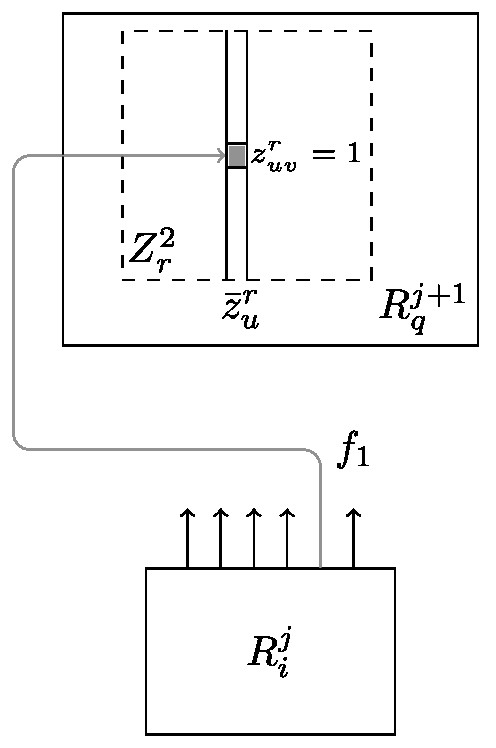
\includegraphics[width=0.3\linewidth]{automata/meas}
	\caption{Определение отношения поглощения на множестве признаков ($f_1\sqsubset f_2$).}
	\label{fig:rb_measure}
\end{figure}

Значение знака предлагается рассматривать как множество правил, каждое из которых соответствует некоторому действию. Правило для простоты представляется в виде пары <<условия "--- эффект действия>> так,~как это принято в искусственном интеллекте. 

Вводится операция $\Lambda$, которая по множеству матриц распознавания $\mathcal Z_k$ признака $f_k$ определяет два набора индексов столбцов матриц из $Z_k$. Первый набор $I_c=\{i_1^c,i_2^c,\dots\}$, $\forall k\ 0\leqslant i_k^c < h$, составляют индексы \textit{столбцов условий}, в которых ненулевые элементы определяют условия проявления признака $f_k$. Второй набор $I_e=\{i_1^e,i_2^e,\dots\}$, $\forall k\ 0\leqslant i_k^e < h$, состоит из индексов  \textit{столбцов эффектов}, в которых ненулевые элементы определяют эффекты проявления признака $f_k$. 

\begin{Def}
	Признаки, для матриц предсказания которых процедура $\Lambda$ выдаёт непустые множества индексов $I_c$ и $I_e$, называются процедурными признаками, остальные "--- объектными признаками.
\end{Def}

Семейство отношений $\{\sqsubset,\sqsubset^1,\sqsubset^2,\dots\}$ пополняется двумя отношениями: $\sqsubset^c$ и $\sqsubset^e$, принадлежность к которым пары признаков $(f_1,f_2)$ свидетельствует о том, что признак $f_1$ присутствует соответственно в столбце условий и эффектов как минимум в одной матрице предсказания процедурного признака $f_2$.

Далее даются определения образа и значения знака. Пусть $S$ "--- множество знаков. Считается, что между множествами $S$ и $\mathcal F$ установлено некоторое взаимно-однозначное соответствие.

\begin{Def}
	Если $f_1$ "--- признак, соответствующий знаку $s_1$, то подмножество $\tilde p(f_1)\subset\mathcal F$ таких признаков, что $\forall f_i\in\tilde p(f_1) f_i\sqsubset f_1$, называется образом знака $s_1$ (признака $f_1$).
\end{Def}

На множестве всех образов $\tilde P$ вводится метрика $\rho_p(\tilde p(f_1),\tilde p(f_2))$, $f_1\dashv R_i^j, f_2\dashv R_u^s$, вычисляемая по следующему правилу:
\[
\rho_p(\tilde p(f_1),\tilde p(f_2))=
\begin{cases}
\infty, & \text{если}\ R_i^j\not=R_u^s,\\
\min\limits_{\substack{Z_r^1\in Z_1\\Z_s^2\in Z_2}}\frac{1}{q\cdot h}\sum\limits_{u=1}^h\|\bar z_u^r-\bar z_u^s\|, & \text{если}\ R_i^j=R_u^s.
\end{cases}
\]

\begin{Def}
	Если $f_1$ "--- признак, соответствующий знаку $s_1$, $f_2$ "--- процедурный признак и $f_1\sqsubset^c f_2$, то $f_2$ называется элементом значения знака $s_1$ (признака $f_1$). Множество всех элементов значения признака $f_1$ будем обозначать $\tilde m(f_1)$.
\end{Def}

На множестве всех значений $\tilde M$ вводится метрика $\rho_m(\tilde m(f_1),\tilde m(f_2))$ следующим образом:
\[
\rho_m(\tilde m_1(f_1),\tilde m_2(f_2 ))=\min\limits_{\substack{f_i\in\tilde m(f_1 )\\f_j\in\tilde m(f_2 )}}\rho_p(\tilde p(f_i ),\tilde p(f_j )).
\]

\begin{algorithm}[hS]
	\caption{Алгоритм $\mathfrak{A}_{pm}$ (часть I)}
	\label{alg:cycle_pm_start}
	\begin{algorithmic}[1]
			\Require $\tilde m^0=\{f_p^0\}, \Psi_p^m, \hat F=dom\ \Psi_p^m\subseteq \mathcal F$;
	\algrule
	\State $Z_p^0 := \{\bar z_1^{c0},\bar z_2^{e0}\}$ "--- матрица предсказания признака $f_p^0$;
	\State $\tilde p^{(0)} := \varnothing$, $\tilde m^{(0)} := \varnothing$;
	\State $R_0\not\in\mathcal R$ "--- фиктивный распознающий блок, для которого $F_0^*=\{f_p^0\}$;
	\State $Z^{(0)} := \varnothing$, $Z_p^{(0)} := \{\bar 0, \bar 0\}$;
	\State $q^{(0)} := 0$, $t := 0$;
	
	\While{$Z_p^{(t)}\not=Z_p$ или $t<|\hat F|$}
		\State $f\in\hat F$ "--- первый не рассмотренный ранее признак; 
		\State $Z=\{\bar z_1,\bar z_2,\dots,\bar z_q\}$ "--- его матрица предсказания;
		\If{$\exists \tilde m=\{f_p\}\in \tilde M$ такое, что $(\tilde p(f),\tilde m)\in\Psi_p^m$, $f_p$ выполним в условиях признака $f_p^0$ и $\nexists f'$ такого, что $f'\in\tilde p^{(t)}$,$\tilde m'=\{f'_p\}\in\tilde M$, $(\tilde p(f'),\tilde m')\in\Psi_p^m$, $f'_p$ конфликтует с $f_p$}\label{alst:find_m}
			\State $\tilde p^{(t+1)}=\tilde p^{(t)}\cup\{f\}$;
			\State $Z_p=\{\bar z_1^{c},\bar z_2^{e}\}$ "--- матрица предсказания признака $f_p$;
	
			\If{$\exists R_i^j$ такой, что $\tilde p^{(t+1)}\subseteq F_i^j$}
				\State $R_i^{j(t+1)}:=R_i^j$;
			\Else
				\State $R_i^{j(t+1)}:=\argmax\limits_{\mathcal R} (F_i^j\cap\tilde p^{(t+1)})$;
				\State $F_i^{j(t+1)}:=F_i^{j(t)}\cup\tilde p^{(t+1)}$;
			\EndIf

		\algstore{algst:store2}
	\end{algorithmic}
\end{algorithm} 

Опыт наблюдения субъекта записывается в виде функции $\Psi_p^m$: $\Psi_p^m(\tilde p)=\tilde m$, в том случае, если $\tilde p\in\tilde P$ является образом некоторого знака $s$, а $\tilde m\in\tilde M$ -- значением того же знака $s$. Строится алгоритм $\mathfrak A_{pm}$ доопределения функции $\Psi_p^m$, обеспечивающий формирование такого образа из множества признаков $\hat F=dom\ \Psi_p^m$, при котором формируемое значение знака стремится к заданному значению $\tilde m^0=\{f_p^0\}$.

\begin{algorithm}[h]
	\caption{Алгоритм $\mathfrak{A}_{pm}$ (часть II)}
	\label{alg:cycle_pm_end}
	\begin{algorithmic}[1]
		\algrestore{algst:store2}
					\State $q^{(t+1)}=\max\{q^{(t)},q\}$;
			\State $Z^{(t+1)}:=\{\bar z_1^{(t+1)},\bar z_2^{(t+1)},\dots \bar z_{q^{(t+1)}}^{(t+1)}\}$, где $\bar z_i^{(t+1)}=\bar z_i^{(t)}\vee \bar z_i$, если $i\leqslant q$ и $i\leqslant q^{(t)}$, $\bar z_i^{(t+1)}=\bar z_i^{(t)}$, если $i>q$ и $\bar z_i^{(t+1)}=\bar z_i$, если $i > q^{(t)}$;
			
			\State $Z_p^{(t+1)}:=\{\bar z_1^{c(t+1)},\bar z_2^{e(t+1)}\}$, где $\bar z_1^{c(t+1)}=\bar z_1^{c(t)}\vee (\bar z_1^c\rightarrow R_0)$, $\bar z_2^{e(t+1)}=\bar z_2^{e(t)}\vee (\bar z_2^e\xrightarrow{\bar z_2^{e0}} R_0)$;
			
			\State $f_p^{(t+1)}$ "--- признак с матрицей предсказания $Z_p^{(t+1)}$;
			
			\State $\tilde m^{(t+1)}=\{f_p^{(t+1)}\}$;
		\EndIf
	
		\State $t=t+1$;
	\EndWhile

	\State $R^*=R_i^{j(t)}$;
	\State $Z^*=Z^{(t)}$;
	\State $\mathcal Z^{*}=\mathcal Z_i^{j(t)}\cup\{Z^*\}$;	
	
	\Return $\Psi_p^m$, доопределённую на паре $(\tilde p, \tilde m)$, где $\tilde p=\tilde p^{(t)}$, $\tilde m=\tilde m^{(t)}$.
	\end{algorithmic}
\end{algorithm}

Для обоснования данного алгоритма доказывается сходимость функциональных значений, которые строятся в процессе его выполнения, к эталонному значению $\tilde m^0$:

\begin{Theorem}[о корректности алгоритма $\mathfrak A_{pm}$]
	Алгоритм $\mathfrak A_{pm}$ корректен, т.~е. элементы последовательности функциональных значений $\langle\tilde m^{(0)},\tilde m^{(1)},\dots,\tilde m^{(t)}\rangle$, которая строится с помощью алгоритма $\mathfrak A_{pm}$ для функционального значения $\tilde m^0$, приближаются к $\tilde m^0$ в смысле введённой на $\tilde M$ метрики.
\end{Theorem}

В \textbf{заключении} диссертационной работы приведены основные результаты, которые выносятся на защиту:
\begin{enumerate}
	\renewcommand\labelenumi{\theenumi.}
	\item Построена модель компонент знака "--- элемента картины мира субъекта деятельности в рамках сегодняшних представлений о функционировании мозга и психики человека.
	\item Построены четыре типа операторов распознавания (два статических оператора, динамический и иерархический операторы) в терминах алгебраической теории для образной компоненты знака.
	\item Доказаны теоремы корректности линейных замыканий множеств построенных в работе операторов распознавания (статических, динамического и иерархического).
	\item Построен алгоритм формирования и связывания двух компонент знака: образа и значения.
	\item Доказана сходимость алгоритма формирования и связывания двух компонент знака.
\end{enumerate}

\newpage
\renewcommand{\refname}{\Large Публикации автора по теме диссертации}
\titleformat{\subsection}[display]{}{}{}{\it}[]
%\titleformat{command}[shape]{format}			   {label}		 {sep}{before}[after]
\nocite{*}
\bibliography{synopsis}						% Подключаем BibTeX-базы

\textbf{Личный вклад соискателя}: в работах 1--6, 8--9, 11--12 автору принадлежат результаты, относящиеся к моделям структурных компонент элемента картины мира субъекта деятельности, к свойствам этих моделей и алгоритмам на их основе.